% ====================================================================
% graphite_ica_ch1_v7-05.tex — Chapter 1 (v7-05)
%   흑연 음극 dQ/dV(ICA) 이론 — v11_final.py 클래스 계산 진행(N0->N9)을
%   절 순서로 삼아 그 진행에 필요한 물리식만 그 순서대로 유도하는 수식 주도판.
%   = "v5 형식(수식 주도)을 v11_final 코드에 맞게 어레인지".
%   식별자/부호는 Anode_Fit_v11_final.py 와 1:1. 그림은 전부 신규 TikZ(영어 ASCII 내부).
%   build: xelatex -interaction=nonstopmode 2-pass (kotex — 한글 verbatim 은 XeLaTeX 전제)
% ====================================================================
\documentclass[11pt,a4paper]{article}
\usepackage[margin=22mm]{geometry}
\usepackage{kotex}
\setmonofont{D2Coding}[Scale=MatchLowercase]
\usepackage{amsmath,amssymb,mathtools,bm}
\usepackage{booktabs,longtable,array}
\usepackage{enumitem}
\usepackage{amsthm}
\usepackage{hyperref}
\usepackage{fancyhdr}
\usepackage{lastpage}
\usepackage{setspace}
\usepackage{tikz}
\usetikzlibrary{positioning,arrows.meta,calc}
\setstretch{1.12}
\setlength{\parskip}{0.45em}\setlength{\parindent}{0pt}\setlength{\headheight}{14pt}
\setlength{\emergencystretch}{2em}
\hypersetup{colorlinks=true, linkcolor=blue, urlcolor=blue, citecolor=blue,
  pdftitle={흑연 음극 dQ/dV 이론: 코드 진행 N0-N9 수식-구동 — Chapter 1 (v7-05)}}
\pagestyle{fancy}\fancyhf{}
\lhead{흑연 음극 $dQ/dV$ 이론 — Ch.1 (v7-05, 코드 진행 N0--N9)}\rhead{\thepage/\pageref{LastPage}}
\renewcommand{\headrulewidth}{0.4pt}

\newtheorem*{keybox}{핵심}
\newtheorem*{codebox}{코드 대응}
\newtheorem*{boundbox}{유효 범위}
\newtheorem*{verifybox}{검산}

\newcommand{\dd}{\mathrm{d}}
\newcommand{\eff}{\mathrm{eff}}
\newcommand{\eq}{\mathrm{eq}}
\newcommand{\app}{\mathrm{app}}
\newcommand{\cell}{\mathrm{cell}}
\newcommand{\bg}{\mathrm{bg}}
\newcommand{\work}{\mathrm{work}}
\newcommand{\rep}{\mathrm{rep}}
\newcommand{\lag}{\mathrm{lag}}
\newcommand{\dis}{\mathrm{dis}}
\newcommand{\chg}{\mathrm{chg}}
\newcommand{\hys}{\mathrm{hys}}
\newcommand{\rxn}{\mathrm{rxn}}
\newcommand{\code}[1]{\texttt{#1}}

\renewcommand{\theequation}{1.\arabic{equation}}
\renewcommand{\thesection}{1.\arabic{section}}
\title{\textbf{\LARGE Chapter 1}\\[0.35em]\Large 흑연 음극 $dQ/dV$ 이론: 한 곡선을 그리는 계산 진행에서 피팅까지 — 코드-진행 수식-구동판}
\author{}
\date{}

\makeatletter
\renewcommand*\l@section[2]{%
  \ifnum \c@tocdepth >\z@
    \addpenalty\@secpenalty
    \addvspace{1.0em \@plus\p@}%
    \setlength\@tempdima{2.3em}%
    \begingroup
      \parindent \z@ \rightskip \@pnumwidth
      \parfillskip -\@pnumwidth
      \leavevmode \bfseries
      \advance\leftskip\@tempdima
      \hskip -\leftskip
      #1\nobreak\hfil
      \nobreak\hb@xt@\@pnumwidth{\hss #2\kern-\p@\kern\p@}\par
    \endgroup
  \fi}
\renewcommand*\l@subsection{\@dottedtocline{2}{2.3em}{3.2em}}
\makeatother

\begin{document}
\maketitle

% ====================================================================
\section*{서론 — 한 곡선을 그리는 계산을 절 순서로}
\addcontentsline{toc}{section}{서론}
% ====================================================================
리튬이온전지 흑연 음극의 \textbf{incremental capacity analysis}(ICA)는 충방전 곡선 $Q(V)$ 의 미분
$\dd Q/\dd V$ 를 본다 \cite{bloom2005,dubarry2012}. 흑연은 staging 상전이(stage
$4\!\to\!3\!\to\!2\mathrm L\!\to\!2\!\to\!1$; $2\mathrm L$ 은 stage-2 의 면내 질서가 풀린 단계)를 거치며
\cite{dahn1991,ohzuku1993,funabiki1999}, 각 전이에서 두 상이 공존하면 전위가 거의 평탄($\dd V_n/\dd q\to0$)이라
좁은 $\dd V$ 에 큰 $\dd Q$ 가 몰려 $\dd Q/\dd V$ 가 치솟는다 — ``전위 평탄 구간 $=$ ICA peak''가 본 장의 대상이다.

본 장은 한 가지 약속으로 다른 ICA 이론서와 갈린다. \textbf{서술의 척추가 한 곡선을 실제로 그리는 계산 코드의 진행 순서다.} 구현(\code{Anode\_Fit\_v11\_final.py})은 실험 조건 한 묶음$(V_\app,\ \text{방향},\ \text{C-rate},\ Q_\cell,\ T)$을 받아 $\dd Q/\dd V$ 한 곡선을 반환한다. 그 내부는 아홉 단계 $N0\!\to\!N9$ 를 순서대로 밟는다 — 조건을 모델 입력으로 바꾸고(N0), 측정 전위에서 분극을 벗기고(N1), 전이별로 평형 중심을 잡고(N2), 충방전 갈림을 중심에 새기고(N3), 폭과 평형 점유를 세우고(N4--N5), 평형 peak 를 읽고(N6), 동역학 지연 길이를 산출하고(N7), 인과 기억으로 꼬리를 만들고(N8), 전이별 기여를 합산해 되돌린다(N9). 본 장의 각 절은 이 노드 하나를 맡아, 그 단계가 무엇을 계산하는지를 \emph{이해하는 데 필요한 물리식만} 그 순서대로 유도한다.

\textbf{관측.}
\begin{quote}\itshape
$\dd Q/\dd V$ 상전이 peak 의 \textbf{위치$\cdot$너비$\cdot$높이}는 \textbf{(a) 온도, (b) 극판 전위, (c) C-rate(전류)}
세 가지에 따라 변한다. 저온$\cdot$고율일수록 peak 의 꼬리가 길어져 다음 peak 와 겹치고, 같은 전이가 충전과 방전에서 서로 다른
전위에 peak 를 남기며(충방전 히스테리시스), 이 갈림에는 전류를 $0$ 으로 줄여도 사라지지 않는 성분이 있다.
\end{quote}

세 인자가 곡선에 들어오는 자리는 코드 진행이 그대로 가리킨다. 온도는 평형 중심 $U_j(T)$(N2)와 폭 $w\propto T$(N4)와 지연 길이의 지수 분모(N7)에, 전위는 평형 점유 logistic 의 인자(N5)와 지연 길이의 유효 장벽(N7)에, C-rate(전류)는 분극(N1)과 지연 길이 $L_V\propto|I|$(N7)에 들어온다. 방전이 본론이고(곡선 진행 부호 $\sigma_d=+1$), 충전은 분극 부호$\cdot$분기 중심$\cdot$꼬리 방향 세 자리만 $\sigma_d=-1$ 로 갈리는 확장이다.

이 장이 닫는 도착점은 둘이다. 하나는 한 줄 합산식 $\dd Q/\dd V = C_\bg+\sum_j Q_j[\text{평형 peak}-\text{지연 꼬리}]$(N9)이고, 다른 하나는 그 식의 모든 기호를 측정 파일에서 정하는 비순환 피팅 사슬이다. 후자는 본 장만 보고 곡선 재현 코드를 짤 수 있을 만큼 컷$\cdot$창$\cdot$회귀 입출력$\cdot$초기값이 닫혀 있어야 한다는 요구(이하 ``재현 가능성'')를 만족하도록 적는다.

흑연 staging 의 갤러리 채움(리튬화 방향 $4\to3\to2\mathrm L\to2\to1$, 방전은 역순)을 그림~\ref{fig:staging} 에 둔다 — 각 stage 전이가 $\dd Q/\dd V$ 에 peak 하나를 남기고, 코드의 전이 목록(\code{GRAPHITE\_STAGING\_LIT}, N9 표~\ref{tab:staging})이 이 네 전이다.

\begin{figure}[t]
\centering
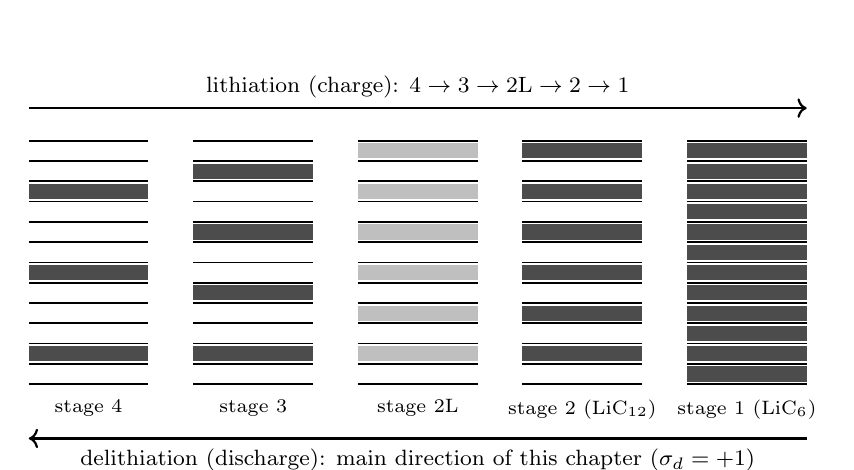
\begin{tikzpicture}[x=0.95cm,y=0.92cm]
% stage 4
\fill[black!70] (0.0,0.315) rectangle (1.6,0.525);
\fill[black!70] (0.0,1.435) rectangle (1.6,1.645);
\fill[black!70] (0.0,2.555) rectangle (1.6,2.765);
\foreach \yy in {0.0,0.28,0.56,0.84,1.12,1.40,1.68,1.96,2.24,2.52,2.80,3.08,3.36}
  {\draw[semithick] (0.0,\yy) -- (1.6,\yy);}
\node[below,align=center] at (0.8,-0.08) {\scriptsize stage 4};
% stage 3
\fill[black!70] (2.2,0.315) rectangle (3.8,0.525);
\fill[black!70] (2.2,1.155) rectangle (3.8,1.365);
\fill[black!70] (2.2,1.995) rectangle (3.8,2.205);
\fill[black!70] (2.2,2.835) rectangle (3.8,3.045);
\foreach \yy in {0.0,0.28,0.56,0.84,1.12,1.40,1.68,1.96,2.24,2.52,2.80,3.08,3.36}
  {\draw[semithick] (2.2,\yy) -- (3.8,\yy);}
\node[below,align=center] at (3.0,-0.08) {\scriptsize stage 3};
% stage 2L
\fill[black!25] (4.4,0.315) rectangle (6.0,0.525);
\fill[black!25] (4.4,0.875) rectangle (6.0,1.085);
\fill[black!25] (4.4,1.435) rectangle (6.0,1.645);
\fill[black!25] (4.4,1.995) rectangle (6.0,2.205);
\fill[black!25] (4.4,2.555) rectangle (6.0,2.765);
\fill[black!25] (4.4,3.115) rectangle (6.0,3.325);
\foreach \yy in {0.0,0.28,0.56,0.84,1.12,1.40,1.68,1.96,2.24,2.52,2.80,3.08,3.36}
  {\draw[semithick] (4.4,\yy) -- (6.0,\yy);}
\node[below,align=center] at (5.2,-0.08) {\scriptsize stage $2\mathrm L$};
% stage 2
\fill[black!70] (6.6,0.315) rectangle (8.2,0.525);
\fill[black!70] (6.6,0.875) rectangle (8.2,1.085);
\fill[black!70] (6.6,1.435) rectangle (8.2,1.645);
\fill[black!70] (6.6,1.995) rectangle (8.2,2.205);
\fill[black!70] (6.6,2.555) rectangle (8.2,2.765);
\fill[black!70] (6.6,3.115) rectangle (8.2,3.325);
\foreach \yy in {0.0,0.28,0.56,0.84,1.12,1.40,1.68,1.96,2.24,2.52,2.80,3.08,3.36}
  {\draw[semithick] (6.6,\yy) -- (8.2,\yy);}
\node[below,align=center] at (7.4,-0.08) {\scriptsize stage 2 ($\mathrm{LiC_{12}}$)};
% stage 1
\foreach \yy in {0.035,0.315,0.595,0.875,1.155,1.435,1.715,1.995,2.275,2.555,2.835,3.115}
  {\fill[black!70] (8.8,\yy) rectangle (10.4,{\yy+0.21});}
\foreach \yy in {0.0,0.28,0.56,0.84,1.12,1.40,1.68,1.96,2.24,2.52,2.80,3.08,3.36}
  {\draw[semithick] (8.8,\yy) -- (10.4,\yy);}
\node[below,align=center] at (9.6,-0.08) {\scriptsize stage 1 ($\mathrm{LiC_6}$)};
\draw[->,thick] (0,3.81) -- (10.4,3.81) node[pos=0.5,above] {\footnotesize lithiation (charge): $4\to3\to2\mathrm L\to2\to1$};
\draw[<-,thick] (0,-0.75) -- (10.4,-0.75) node[pos=0.5,below] {\footnotesize delithiation (discharge): main direction of this chapter ($\sigma_d=+1$)};
\end{tikzpicture}
\caption{흑연 staging 의 갤러리 채움 도식. 수평선이 그래핀 층, 음영 띠가 리튬이 든 층간
갤러리다. 채울수록 stage 번호가 줄어 stage 1($\mathrm{LiC_6}$, 완전 채움)에 닿고, 각 stage 전이가
$\dd Q/\dd V$ 에 peak 하나를 남긴다. stage $2\mathrm L$ 은 갤러리 안이 희박하고 면내 질서가 풀린(liquid-like)
단계라 옅게 표시했다. 코드의 전이 목록이 표~\ref{tab:staging} 의 네 전이($4\!\to\!3$, $3\!\to\!2\mathrm L$, $2\mathrm L\!\to\!2$, $2\!\to\!1$)다.}
\label{fig:staging}
\end{figure}

\tableofcontents
\newpage

% ====================================================================
\section{기호와 규약 — 코드 진행 N0--N9 의 사전}\label{sec:notation}
% ====================================================================
표는 본 장의 절 순서 $=$ 코드 노드 순서($N0\!\to\!N9$)대로 배열된 사전이다. 모든 기호$\cdot$부호는 구현(\code{Anode\_Fit\_v11\_final.py})과 1:1 이며, 박스 결과식과 코드 식별자를 나란히 둔다.

\textbf{전이 인덱스.} $j=1,\dots,N_p$($N_p\approx3$--$4$; 흑연은 표~\ref{tab:staging} 의 $4$ 전이). 전이 $j$ 마다 진행률 $\xi_j$(방전 시 $0\to1$ 로 증가, 탈리튬화 진행). 코드의 전이 dict 가 곧 $j$ 다.

\textbf{부호 규약(★최우선).} 방향 부호 $\sigma_d\in\{+1,-1\}$ — 방전 $+1$, 충전 $-1$(코드 \code{s}, \code{\_direction\_to\_sigma}). 평형 곡선 자체는 진행 방향에 불변인 상태함수이고, $\sigma_d$ 가 \emph{값}을 바꾸는 자리는 셋뿐이다 — \textbf{(1) 분극 부호}(N1: $V_n=V_\app-\sigma_d|I|R_n$), \textbf{(2) 분기 중심}(N3: $U_j^d=U_j+\tfrac12\sigma_d h_\eta\gamma\,\Delta U_j^\hys$), \textbf{(3) 꼬리 방향}(N8: 충전은 격자 역전). 방전 기준 핵심 부호 사슬 — $V$ 상승 $\Rightarrow$ 탈리튬화 진행 $\xi$ 증가 $\Rightarrow$ 평형 peak 양수, 충전 $\dd Q/\dd V$ 는 방전의 거울(양수 유지). 이 사슬은 §\ref{sec:summation} 까지 전건 유지된다.

\begin{longtable}{p{0.15\textwidth} p{0.13\textwidth} p{0.40\textwidth} p{0.20\textwidth}}
\toprule 기호 & 단위 & 의미 & 코드 식별자 \\ \midrule \endhead
\multicolumn{4}{l}{\emph{— N0 실험 조건 $\to$ 모델 입력 (§\ref{sec:input}) —}}\\
$\sigma_d$ & --- & 방향 부호(방전 $+1$/충전 $-1$) & \code{s}, \code{sigma\_d} \\
$|I|$ & A & 전류 크기 $=$ C-rate$\cdot Q_\cell$ & \code{I\_abs} \\
$Q_\cell$ & C & 셀 용량(전하) & \code{Q\_cell} \\
$T$ & K & 온도(스칼라 또는 $T(V)$ 배열) & \code{T} \\
$q$ & --- & 무차원 용량 $=Q/Q_\cell$ & --- \\
\multicolumn{4}{l}{\emph{— N1 분극 (§\ref{sec:polar}) —}}\\
$V_\app$ & V & 인가(측정) 전위 격자 & \code{V\_app} \\
$V_n$ & V & 내부(열역학) 전위 $=V_\app-\sigma_d|I|R_n$ & \code{V\_n} \\
$R_n$ & $\Omega$ & 직렬 분극 저항(lumped) & \code{Rn} \\
$V_\work$ & V & 작업 격자(꼬리 여유 pad) & \code{V\_work} \\
$C_\bg$ & C/V & 배경 미분용량 & \code{Cbg} \\
\multicolumn{4}{l}{\emph{— N2 평형 중심 (§\ref{sec:center}) —}}\\
$U_j(T)$ & V & 전이 $j$ 평형 중심 $=(-\Delta H_\rxn+T\Delta S_\rxn)/F$ & \code{func\_U\_j} \\
$\Delta H_\rxn,\Delta S_\rxn$ & {\footnotesize J/mol;\,J/(mol\,K)} & 삽입 반응 엔탈피$\cdot$엔트로피 & \code{dH\_rxn,dS\_rxn} \\
\multicolumn{4}{l}{\emph{— N3 히스테리시스 분기 (§\ref{sec:hys}) —}}\\
$\Omega_j$ & J/mol & 정규용액 상호작용($>2RT$ 면 상분리) & \code{Omega} \\
$\gamma_j$ & --- & 분기 축소 인자 $0\le\gamma_j\le1$ & \code{gamma} \\
$h_\eta$ & --- & 부분 cycle 인자(기본 $1$) & \code{h\_eta} \\
$\Delta U_j^\hys$ & V & spinodal 상한 분기 gap & \code{func\_dU\_hys} \\
$U_j^d$ & V & 분기 중심 $=U_j+\tfrac12\sigma_d h_\eta\gamma\Delta U_j^\hys$ & \code{func\_U\_branch} \\
\multicolumn{4}{l}{\emph{— N4--N6 폭$\cdot$평형 점유$\cdot$평형 peak (§\ref{sec:width}--\ref{sec:eqpeak}) —}}\\
$w_j$ & V & 전이 폭 $=nRT/F$(옵션 $w^\eff$) & \code{func\_w/func\_w\_eff} \\
$n$ & --- & 폭 다중도(기본 $1$) & \code{n} \\
$\xi_{\eq,j}$ & --- & 평형 점유 $=\mathrm{logistic}[\sigma_d(V_n-U)/w]$ & \code{func\_ksi\_eq} \\
$Q_j$ & C & 전이 $j$ 용량 가중 & \code{Q} \\
\multicolumn{4}{l}{\emph{— N7 동역학 지연 길이 (§\ref{sec:tail}) —}}\\
$\mathcal A$ & J/mol & 컷 affinity $=\min(z_\mathrm{cut}\,nRT,\ A_\mathrm{cap}RT)$ & \code{A} \\
$\chi,\chi_d$ & --- & 전달 계수, 방향형(방전 $\chi$/충전 $1-\chi$) & \code{chi/func\_chi\_d} \\
$\Delta H_a,\Delta S_a$ & {\footnotesize J/mol;\,J/(mol\,K)} & 활성화 엔탈피$\cdot$엔트로피 & \code{dH\_a,dS\_a} \\
$\Delta H_a^\eff$ & J/mol & 유효 장벽 $=\Delta H_a-\chi_d\Omega$ & \code{func\_dH\_a\_eff} \\
$L_q,\ L_V$ & ---;\,V & 용량축$\cdot$전압축 지연 길이 & \code{func\_L\_q}, \code{lag\_len\_V} \\
$|\dd V/\dd q|_{q_a}$ & V & 컷점 OCV 기울기($L_q\!\to\!L_V$) & \code{dVdq\_qa} \\
$z_\mathrm{cut},A_\mathrm{cap}$ & ---;\,--- & 컷 $z=\mathcal A/(nRT)$, 상한 배수 & \code{z\_cut,A\_cap\_RT} \\
\multicolumn{4}{l}{\emph{— N8--N9 인과 꼬리$\cdot$합산 (§\ref{sec:memory}--\ref{sec:summation}) —}}\\
$\xi_\lag$ & --- & 인과 저역통과(지연) 점유 & \code{occ\_lagged} \\
$g_\mathrm{step}$ & V & 작업 격자 간격 & \code{grid\_step} \\
$R,F,k_B,h$ & {\footnotesize J/(mol\,K),C/mol,J/K,J\,s} & 기체상수, Faraday, Boltzmann, Planck & \code{R,F,kB,h} \\
\bottomrule
\end{longtable}

이제 노드 순서대로 내려간다. 각 절은 앞 절에서 받은 양을 명시하고(도입), 절 끝에서 다음 노드로 무엇을 넘기는지를 적는다(마무리).

% ====================================================================
\section{N0--N1 — 실험 조건에서 내부 전위 $V_n$ 으로}\label{sec:input}\label{sec:polar}
% ====================================================================
계산의 입구는 facade \code{curve(V\_app, direction, c\_rate, Q\_cell, T)} 이고, 이 함수가 하는 일은 두 가지 환산뿐이다 — 방향 문자열을 부호로($\text{direction}\to\sigma_d$), C-rate 를 전류 크기로($|I|=\text{C-rate}\cdot Q_\cell$). 그다음 코어 \code{dqdv} 에 넘긴다. 본 절은 이 환산(N0)과, 코어가 맨 처음 하는 분극 보정(N1)을 닫는다.

\subsection{N0 — 조건을 모델 입력으로}
실험은 ``$0.2$C 로 방전하며 측정 전위 $V_\app$ 를 읽는다''처럼 적히지만, 물리식이 받는 입력은 부호$\cdot$전류 크기$\cdot$온도다. 방향 부호는
\begin{equation}
\sigma_d=\begin{cases}+1 & \text{방전(discharge, delithiation)}\\ -1 & \text{충전(charge, lithiation)}\end{cases}
\label{eq:sigma}
\end{equation}
이고(코드 \code{\_direction\_to\_sigma}: 문자열 또는 부호 입력을 $\pm1$ 로), 전류 크기는 율 정의 ``전류 $=$ 율 $\times$ 용량''에서
\begin{equation}
|I|=\text{C-rate}\cdot Q_\cell\qquad(\ge0)
\label{eq:Iabs}
\end{equation}
다(\code{I\_abs} 를 직접 주면 그 값이 우선). 무차원 용량 좌표는 $q=Q/Q_\cell=\int|I|\,\dd t/Q_\cell$ 로, 곡선의 진행을 잰다. 이 셋$(\sigma_d,|I|,T)$ 과 $Q_\cell$ 이 코어의 입력이다.

\subsection{N1 — 분극: 측정 전위에서 열역학 전위 벗기기}
관측 전위 $V_\app$ 는 평형 전위가 아니다. 전류가 흐르면 직렬 저항 $R_n$ 에 분극이 걸려, 측정값이 내부(열역학) 전위에서 어긋난다. 어긋남의 \emph{부호}가 방향에 달렸다 — 방전($\sigma_d=+1$, 산화)은 분극이 측정 전위를 내부 전위보다 \emph{올리고}, 충전은 내린다. 이 한 줄이 N1 의 전부다:
\begin{equation}
\boxed{\;V_n\;=\;V_\app\;-\;\sigma_d\,|I|\,R_n\;.}
\label{eq:vn}
\end{equation}
부호를 검산하면 — 방전 시 $\sigma_d|I|R_n>0$ 이라 $V_n<V_\app$(측정 전위가 평형보다 높게 읽힘을 벗겨 낮춤), 충전 시 $V_n>V_\app$. $|I|\to0$ 또는 $R_n=0$ 이면 $V_n=V_\app$ 로 측정$=$내부가 합치한다. 분극은 $|I|$ 에 선형인 lumped 근사이며, 계면 과전압을 내부 전위에 흡수한 그림이다 — 율속이 고상 재배열$\cdot$핵생성에 지배될 때 타당하다.

\begin{codebox}
\code{dqdv} 의 첫 실효 줄이 식~\eqref{eq:vn} 이다: \code{V\_n = V\_in - sigma\_d * I\_abs * self.Rn}. 이후 모든 평형$\cdot$동역학 계산은 $V_n$ 위에서 돌고, 마지막에 \code{np.interp(V\_n, V\_work, dqdv\_work)} 로 측정축에 되앉힌다(N9).
\end{codebox}

\subsection{작업 격자 $V_\work$ — 꼬리가 양쪽으로 들어오도록}
N8 의 인과 꼬리는 격자 위 합성곱이라, peak 가 격자 끝에 너무 가까우면 꼬리가 잘린다. 그래서 코드는 측정 범위 $[v_\mathrm{lo},v_\mathrm{hi}]$ 양쪽에 여유(pad)를 둔 균일 작업 격자를 만든다:
\begin{equation}
V_\work=\mathrm{linspace}\big(v_\mathrm{lo}-p_\mathrm{lo}\,\Delta v,\ \ v_\mathrm{hi}+p_\mathrm{hi}\,\Delta v,\ \ n_\work\big),\qquad
\Delta v=\max(v_\mathrm{hi}-v_\mathrm{lo},\ \epsilon_v),
\label{eq:vwork}
\end{equation}
패딩 분율 $p_\mathrm{lo}=p_\mathrm{hi}=0.15$(\code{grid\_pad\_lo/hi}), 점 수 $n_\work=\max(2048,\ 2|V_n|)$(\code{n\_work\_min}), $\Delta v$ 의 하한 $\epsilon_v$(\code{v\_span\_floor})는 단일점 입력에서 폭 $0$ 발산을 막는다. 격자 간격 $g_\mathrm{step}=V_\work[1]-V_\work[0]$ 은 N8 합성곱의 보폭이다. 비등온 $T(V)$ 면 작업 격자에 $T_\work$ 를 보간하고, 대표 온도 $T_\rep=\overline{T_\work}$ 를 전이당 상수(N7 지연 길이) 평가에 쓴다. 배경은 $C_\bg$(상수 또는 $V$ 함수)로 작업 격자에 깔아 둔다.

\medskip
\emph{넘김.} N1 은 내부 전위 $V_n$ 과 작업 격자$(V_\work,g_\mathrm{step},T_\work,T_\rep)$, 배경 $C_\bg$ 를 만들었다. 이제 전이 루프(N2--N8)가 전이 $j$ 마다 돌며 평형 종과 꼬리를 쌓는다. 첫 단계는 전이의 평형 중심 $U_j(T)$ 다.

% ====================================================================
\section{N2 — 평형 중심 $U_j(T)$ — 열역학에서}\label{sec:center}
% ====================================================================
전이 루프의 첫 줄은 평형 중심을 정한다 — 코드는 \code{U} 직접 지정이 있으면 그것을, 없으면 열역학 환산 \code{func\_U\_j(T, dH\_rxn, dS\_rxn)} 을 쓴다. 이 절은 그 환산식이 어디서 나오는지를, 곡선에 필요한 만큼만 유도한다. $V_n$ 은 N1 에서 받았고, 이 절은 그 축 위에 전이의 중심을 놓는다.

\subsection{$G$ 와 $\mu$ — 평형의 언어}
등온$\cdot$등압 계(전지)에서 자발성$\cdot$평형을 판정하는 퍼텐셜은 Gibbs 자유에너지 $G\equiv H-TS$ 이고, 자발 변화는 $G$ 감소 방향$\cdot$평형은 $G$ 극소다. 입자 1몰 변화당 $G$ 변화가 화학퍼텐셜이다:
\begin{equation}
\mu\;\equiv\;\frac{\partial G}{\partial n}\Big|_{T,P}.
\label{eq:mudef}
\end{equation}
두 장소의 $\mu$ 일치가 입자 교환 평형이다. 삽입 리튬을 ``동등한 자리에 차고 비는'' 격자기체로 보면, 점유율 $\theta$ 에서 화학퍼텐셜은 기준 몫$\cdot$섞임 엔트로피 몫$\cdot$상호작용 몫의 셋으로 닫힌다(상호작용 $\Omega$ 는 N3 에서 살리고, 여기 N2 는 그 결과의 중심만 쓴다):
\begin{equation}
\mu_{\mathrm{Li}}(\theta)=\mu^0+RT\ln\frac{\theta}{1-\theta}+\Omega\,(1-2\theta).
\label{eq:mu}
\end{equation}
로그 항은 섞임 엔트로피($\theta\to0$ 에서 $\mu\to-\infty$, 채울수록 단조 상승), $\Omega$ 항은 상호작용이다. N2 가 정하는 ``중심''은 이 식의 기준 몫과 전기 일이 만드는 평형 전위이고, 조성 의존(로그$\cdot\Omega$)은 N5(폭$\cdot$점유)와 N3(분기)이 받는다.

\subsection{삽입 반응의 평형 조건 — $\Delta G=-FU$}
리튬은 Li$^+$ 와 $e^-$ 로 갈라져 드나들므로 값어치에 전기 일이 더해진다(전기화학 퍼텐셜 $\tilde\mu=\mu+zF\phi$). 삽입 반응 $\mathrm{Li}^++e^-+[\,]\rightleftharpoons\mathrm{Li}_{(\text{흑연})}$ 의 평형 조건 $\tilde\mu_{\mathrm{Li}^+}+\tilde\mu_{e^-}=\tilde\mu_{\mathrm{Li}}$ 에서, 전위 의존은 전자 항 $-FV$ 하나뿐이고 나머지는 주어진 $T$ 에서 상수다. 그 상수 덩이를 $FU^0$ 로 묶고 기준 몫까지 중심에 흡수해 $U\equiv U^0-\mu^0/F$ 로 재정의하면 평형 조건이
\begin{equation}
\mu_{\mathrm{Li}}(\theta_\eq)=\mu^0-F\,(V-U),
\qquad\text{곧}\qquad
\Delta G_j\;=\;-\,F\,U_j
\label{eq:eqcond}
\end{equation}
형태가 된다($s=+1$ 방전 규약을 정의에 고정). $U_j$ 는 비배치 몫 자유에너지를 전위로 환산한 양이라는 지위를 갖는다. 부호 — $V$ 상승(전자 값어치 하락) $\Rightarrow$ 평형 점유 하강, 곧 ``$V$ 를 올리면 탈리튬화''가 이 한 식에 들어 있다(N5 logistic 의 부호가 이것을 잇는다).

\subsection{온도 의존 — $U_j(T)$ 의 닫힌 꼴}
중심의 온도 의존은 Gibbs 항등식 $\partial\Delta G/\partial T|_P=-\Delta S$ 와 식~\eqref{eq:eqcond} 의 $\Delta G_j=-FU_j$ 를 잇는다:
\begin{equation}
\Delta G_j=-F\,U_j,\qquad
\frac{\partial\Delta G_j}{\partial T}=-\Delta S_{\rxn,j}
\quad\Longrightarrow\quad
\frac{\partial U_j}{\partial T}=\frac{\Delta S_{\rxn,j}}{F}.
\label{eq:dUdT}
\end{equation}
$\Delta G_j=\Delta H_{\rxn,j}-T\Delta S_{\rxn,j}$ 를 식~\eqref{eq:eqcond} 의 $\Delta G_j=-FU_j$ 에 넣어 $U_j$ 로 풀면 N2 의 결과식이 닫힌다:
\begin{equation}
\boxed{\;U_j(T)\;=\;\frac{-\Delta H_{\rxn,j}+T\,\Delta S_{\rxn,j}}{F}\;.}
\label{eq:Uj}
\end{equation}
이것이 \code{func\_U\_j} 다. 비등온이면 $T$ 가 배열이라 $U_j$ 도 작업 격자 위 배열로 나온다(코드는 \code{T\_work} 를 그대로 넣는다).

\begin{verifybox}
\textbf{부호$\cdot$수치.} $\Delta H_\rxn<0$(발열 삽입)이라 $-\Delta H_\rxn>0$ 이 중심을 양의 전위로 올린다. 표~\ref{tab:staging} 의 stage $2\!\to\!1$: $\Delta H_\rxn=-13.0$ kJ/mol, $\Delta S_\rxn=-16$ J/(mol\,K) 에서 $U_j(298)=(13000+298\cdot(-16))/96485=(13000-4768)/96485\approx0.085$ V — 목표 $0.085$ V 와 합치. $|\Delta S_\rxn|\sim$ 수십 J/(mol\,K) 라 $|\partial U_j/\partial T|\sim0.01$--$0.1$ mV/K, $30$ K 창에서 수 mV — 다온도 피팅에서 온도마다 $U_j(T)$ 를 따로 읽어야 하는 이유다 \cite{reynier2004}.
\end{verifybox}

\medskip
\emph{넘김.} N2 는 전이의 평형 중심 $U_j(T)$ 를 정했다. 코드는 곧장 N3 의 분기 보정을 더하지만, 분기는 상호작용 $\Omega$ 가 켜진($\gamma\ne0$) 전이에만 작동하는 확장이다. 방전 본론을 먼저 닫기 위해 본 장은 분기 없는 중심($U_j^d\to U_j$)으로 N4--N6 의 평형 종을 세운 뒤, N3 에서 분기를 그 중심 위에 얹는다. 다음 절은 그 종의 폭과 점유를 유도한다.

% ====================================================================
\section{N4--N5 — 폭 $w$ 와 평형 점유 $\xi_\eq$ (logistic)}\label{sec:width}\label{sec:logistic}
% ====================================================================
중심 $U_j$ 를 받아, 이 절은 그 둘레의 평형 점유 곡선을 세운다 — 코드의 \code{func\_w}(폭)와 \code{func\_ksi\_eq}(logistic). 평형 점유는 ``주어진 전위에서 자리가 얼마나 차 있나''이고, 그 곡선의 부호$\cdot$중심$\cdot$폭이 곧 peak 의 부호$\cdot$위치$\cdot$너비가 된다.

\subsection{logistic 의 유도 — 정$\cdot$역 속도의 균형}
평형 점유는 정$\cdot$역 두 방향 사건 속도가 같아지는 정지점이다. 전이상태 이론의 속도식(§\ref{sec:tail} 에서 본격 사용)에서, 구동력 $\mathcal A_j$ 는 평형 전위 $U_j$ 에서 벗어난 전기 항이다:
\begin{equation}
\mathcal A_j\;=\;\sigma_d\,F\,(V_n-U_j).
\label{eq:affinity}
\end{equation}
정$\cdot$역은 같은 전이상태(고개)를 지나고, 고개의 분율 위치 $\chi\in[0,1]$ 에 대해 정방향 장벽은 $\chi\mathcal A_j$ 만큼 낮아지고 역방향은 $(1-\chi)\mathcal A_j$ 만큼 높아진다(Butler--Volmer 형 \cite{bardfaulkner,evanspolanyi1938}). 자리당 속도의 비는 $\chi$ 가 상쇄되어 두 골짜기 자유에너지 차의 Boltzmann 점유비와 같다(detailed balance \cite{bazant2013}):
\begin{equation}
\frac{r_j^+}{r_j^-}=\exp\!\Big[\frac{\mathcal A_j}{RT}\Big].
\label{eq:db}
\end{equation}
정방향은 찬 자리($1-\xi_j$)에서, 역방향은 빈 자리($\xi_j$)에서 출발하므로 운동방정식 $\dd\xi_j/\dd t=r_j^+(1-\xi_j)-r_j^-\xi_j$ 의 정지점($\dd\xi_j/\dd t=0$)에서 $r_j^+(1-\xi_\eq)=r_j^-\xi_\eq$, 곧
\begin{equation}
\frac{\xi_{\eq,j}}{1-\xi_{\eq,j}}=\frac{r_j^+}{r_j^-}=e^{\mathcal A_j/RT}.
\label{eq:stationary}
\end{equation}
$\mathcal A_j=\sigma_dF(V_n-U_j)$ 를 넣어 $\xi_{\eq,j}$ 로 풀면 logistic 이 닫힌다:
\begin{equation}
\boxed{\;\xi_{\eq,j}(V_n,T)=\frac{1}{1+\exp\!\big[-\sigma_d(V_n-U_j)/w_j\big]}\;,\qquad
w_j=\frac{RT}{F}\ \text{(이상 극한)}\;.}
\label{eq:logistic}
\end{equation}
이것이 \code{func\_ksi\_eq} 다. 코드는 오버플로 방지를 위해 $z\equiv\sigma_d(V_n-U)/w$ 의 부호로 두 동등 표현을 가른다($z\ge0$ 면 $1/(1+e^{-z})$, $z<0$ 면 $e^z/(1+e^z)$) — 같은 함수의 수치 안전형이다.

\subsection{부호 검산 — 방향이 종의 부호를 지킨다}
방전($\sigma_d=+1$)에서 $V_n\uparrow\Rightarrow z\uparrow\Rightarrow\xi_\eq\uparrow$ — ``전위를 올리면 탈리튬화 진행 $\xi$ 가 증가''(N2 의 식~\eqref{eq:eqcond} 부호와 합치). 충전($\sigma_d=-1$)에서는 $V_n\downarrow\Rightarrow\xi_\eq\uparrow$. 어느 방향이든 $\xi_\eq$ 는 진행 방향으로 $0\to1$ 증가하고, 중심 $V_n=U_j$ 에서 $\tfrac12$, 양 극한에서 $0$ 과 $1$ 이다. 이 단조 증가가 다음 절의 평형 peak 를 \emph{양수}로 만든다(방향 불변).

\subsection{폭 $w$ — 이상 극한과 $\Omega$ 좁힘}
폭 척도는 logistic 의 가파름을 정한다. 이상 극한은 $w_j=nRT/F$ 이고(다중도 $n$, 기본 $1$; \code{func\_w}), 상호작용이 켜지면 종이 좁아진다. 정규용액 등온선의 중심 기울기를 이상 logistic 과 맞추면 유효 폭이
\begin{equation}
w_j^\eff=\frac{RT}{F}\Big(1-\frac{\Omega_j}{2RT}\Big)
\label{eq:weff}
\end{equation}
로 나온다(\code{func\_w\_eff}). $\Omega_j\to2RT$ 에서 폭이 $0$(종이 무한히 가팔라짐 — plateau 신호), $\Omega_j=0$ 에서 $RT/F$ 회복. 코드는 $w^\eff$ 가 $0$ 으로 떨어져 발산하지 않도록 $\text{floor\_frac}\cdot RT/F$ 하한으로 클립한다(\code{w\_eff\_floor\_frac}$=0.05$). 다만 폭은 기본적으로 $n,w$ 직접 지정이 우선이고, $\Omega$ 좁힘은 \code{use\_w\_eff} 를 명시로 켤 때만 들어온다(\code{\_width}). 분기 영역의 실측 폭은 평형 예측이 아니라 입자 분포 broadening$\cdot$동역학 꼬리가 만드는 현상학 값이므로, 폭을 피팅 자유도로 두는 것이 기본이다.

\begin{figure}[t]
\centering
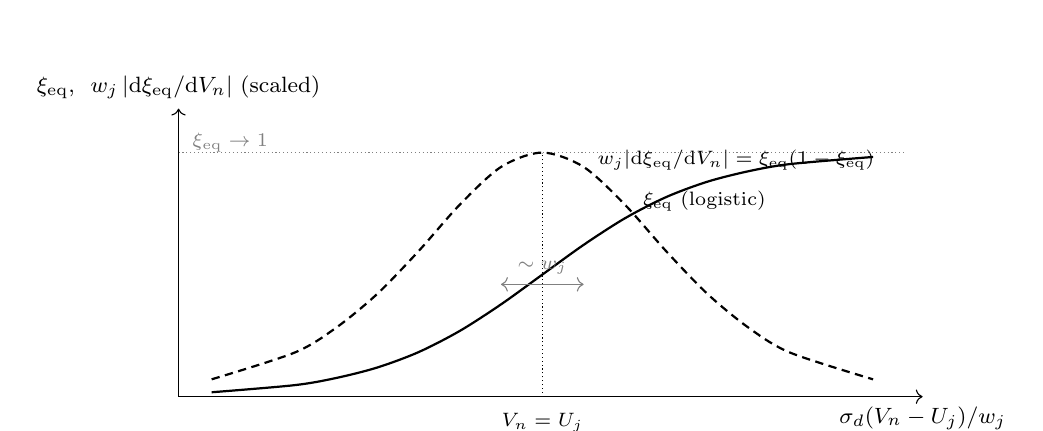
\begin{tikzpicture}[x=1.05cm,y=3.1cm]
\draw[->] (-4.4,0) -- (4.6,0) node[below] {\footnotesize $\sigma_d (V_n-U_j)/w_j$};
\draw[->] (-4.4,0) -- (-4.4,1.18) node[above] {\footnotesize $\xi_\eq$, \ $w_j\,|\dd\xi_\eq/\dd V_n|$ (scaled)};
\draw[gray,densely dotted] (-4.4,1) -- (4.4,1);
\node[right,gray] at (-4.35,1.04) {\scriptsize $\xi_\eq\to1$};
% logistic xi_eq
\draw[thick] plot[smooth] coordinates {(-4,0.018) (-3,0.047) (-2.5,0.076) (-2,0.119) (-1.5,0.182) (-1,0.269) (-0.5,0.378) (0,0.5) (0.5,0.622) (1,0.731) (1.5,0.818) (2,0.881) (2.5,0.924) (3,0.953) (4,0.982)};
% bell xi(1-xi) scaled to 1 at center (max 0.25 -> x4)
\draw[thick,densely dashed] plot[smooth] coordinates {(-4,0.071) (-3,0.180) (-2.5,0.281) (-2,0.420) (-1.5,0.595) (-1,0.786) (-0.5,0.941) (0,1.0) (0.5,0.941) (1,0.786) (1.5,0.595) (2,0.420) (2.5,0.281) (3,0.180) (4,0.071)};
\draw[densely dotted] (0,0) -- (0,1.0);
\node[below] at (0,-0.03) {\scriptsize $V_n=U_j$};
\node[right] at (1.1,0.80) {\scriptsize $\xi_\eq$ (logistic)};
\node[right] at (0.55,0.97) {\scriptsize $w_j|\dd\xi_\eq/\dd V_n|=\xi_\eq(1-\xi_\eq)$};
\draw[<->,gray] (-0.5,0.46) -- (0.5,0.46);
\node[gray,above] at (0,0.46) {\scriptsize $\sim w_j$};
\end{tikzpicture}
\caption{평형 점유 logistic~\eqref{eq:logistic}(실선)과 그 미분 종~\eqref{eq:dxidV}(파선, 중심값 $1$ 로 정규화 — 실제 최대는 $\tfrac14$). 가로축은 방향 정규화 $\sigma_d(V_n-U_j)/w_j$ 라 충$\cdot$방전 공통이다. 중심 $V_n=U_j$ 에서 $\xi_\eq=\tfrac12$$\cdot$종이 최대, 종의 반높이 폭이 $\sim w_j$. 종은 어느 방향에서도 양수(peak 부호 불변).}
\label{fig:logistic}
\end{figure}

\medskip
\emph{넘김.} N4--N5 는 중심 $U_j$ 둘레에 양수$\cdot$단조 종 모양 평형 점유 $\xi_\eq$ 와 폭 $w_j$ 를 세웠다. 다음 N6 은 이 종을 미분해 $|I|\to0$ 극한의 평형 peak 를 읽는다.

% ====================================================================
\section{N6 — 평형 peak ($|I|\to0$ 한계)}\label{sec:eqpeak}
% ====================================================================
관측 ICA 가 전이별 기여의 합이라는 것은 전하 보존에서 나온다. 전이 진행률 $\xi_j$ 의 전위 미분이 ICA 에 들어오므로($\dd Q/\dd V_n=C_\bg+\sum_j Q_j\,\dd\xi_j/\dd V_n$ — N9 에서 합산), 평형 추종이면 그 자리에 평형 종의 미분이 들어간다. 이 절은 그 미분을 닫고, 코드의 \code{equilibrium()} 기준선이 곧 이 식임을 보인다. $\xi_\eq$ 와 $w_j$ 는 N4--N5 에서 받았다.

\subsection{logistic 의 미분 — 종 모양}
식~\eqref{eq:logistic} 을 $z\equiv\sigma_d(V_n-U_j)/w_j$ 로 치환해 $\xi_\eq=(1+e^{-z})^{-1}$ 를 미분하면 종 항등식이 나온다:
\begin{equation}
\frac{\dd\xi_\eq}{\dd z}
=\frac{e^{-z}}{(1+e^{-z})^2}
=\underbrace{\frac{1}{1+e^{-z}}}_{\xi_\eq}\cdot
\underbrace{\frac{e^{-z}}{1+e^{-z}}}_{1-\xi_\eq}
=\xi_\eq(1-\xi_\eq).
\label{eq:belliden}
\end{equation}
연쇄율 $\dd z/\dd V_n=\sigma_d/w_j$ 를 곱하면 평형 종 미분이 닫힌다:
\begin{equation}
\boxed{\;\frac{\dd\xi_{\eq,j}}{\dd V_n}=\frac{\sigma_d\,\xi_{\eq,j}(1-\xi_{\eq,j})}{w_j}\;.}
\label{eq:dxidV}
\end{equation}
$\xi(1-\xi)$ 는 $\xi=\tfrac12$ 에서 최대 $\tfrac14$ 인 종이고(그림~\ref{fig:logistic} 파선), 앞의 $\sigma_d$ 와 N9 의 부호 정렬이 만나 ICA 기여를 \emph{양수}로 만든다 — 방전$\cdot$충전 어느 쪽이든 peak 는 양수다. 이것이 ★부호 사슬의 핵심 마디다.

\subsection{평형 peak 의 세 양과 코드 기준선}
식~\eqref{eq:dxidV} 를 ICA 합산에 넣으면 전이 하나의 평형 기여가
\begin{equation}
Q_j\,\frac{\dd\xi_{\eq,j}}{\dd V_n}\Big|_{|\sigma_d|=1}
=\frac{Q_j\,\xi_{\eq,j}(1-\xi_{\eq,j})}{w_j}
\label{eq:eqcontrib}
\end{equation}
이고($\sigma_d^2=1$ 로 부호가 사라져 항상 양수), 종에서 peak 의 세 양이 읽힌다:
\begin{equation}
V_\mathrm{peak}=U_j(T),\qquad
\Big(\frac{\dd Q}{\dd V_n}\Big)^\mathrm{net}_{\max}=\frac{Q_j}{4w_j},\qquad
\int\Big(\frac{\dd Q}{\dd V_n}-C_\bg\Big)\dd V_n=Q_j.
\label{eq:eqpeak}
\end{equation}
위치 $=$ 중심 $U_j$, 순높이 $=Q_j/(4w_j)$, 배경 차감 면적 $=Q_j$($\int_0^1\dd\xi_\eq=1$). 코드의 \code{equilibrium(V\_n, T)} 메서드가 정확히 이 합이다:
\begin{equation}
\code{equilibrium}\;=\;C_\bg+\sum_j Q_j\,\frac{\xi_{\eq,j}(1-\xi_{\eq,j})}{w_j}.
\label{eq:equilcode}
\end{equation}
이것이 $|I|\to0$ 의 기준선이며 충방전 방향 불변$\cdot$히스 미반영이다 — 전류가 흐를 때의 변화를 이 기준선으로부터의 이탈로 읽는다(N7--N8).

\begin{verifybox}
\textbf{수치$\cdot$극한.} $Q_j=0.5\,Q_\cell$, $w_j=12$ mV 면 순높이 $Q_j/(4w_j)=0.5/(0.048)\approx10.4\,Q_\cell/\mathrm V$, 면적 $=0.5\,Q_\cell$. 극한 — $w\to0$ 에서 높이 발산$\cdot$면적 불변(이상 plateau 선), $T$ 상승 시 $w\propto T$ 라 종이 낮고 넓어진다(면적 보존). \code{dqdv} 의 저율 분기(\code{lag\_len\_V} 가 sub-grid)가 정확히 이 종을 직접 쓴다.
\end{verifybox}

\medskip
\emph{넘김.} N6 은 평형 peak 기준선을 닫았다. 이제 본론 확장이 둘 남았다 — 충방전이 중심을 가르는 분기(N3)와, 전류가 종에 꼬리를 다는 동역학(N7--N8). 코드 진행상 분기가 먼저이므로 N3 으로 간다.

% ====================================================================
\section{N3 — 히스테리시스 분기 $U_j^d$}\label{sec:hys}
% ====================================================================
방전 본론(N4--N6)은 단일 중심 $U_j$ 위에서 닫혔다. 이 절은 충전과 방전이 서로 다른 준안정 가지를 과주행해 중심이 갈리는 현상을 — 상호작용 $\Omega$ 가 켜진 전이에 한해 — 닫힌 식으로 유도한다. 코드는 전이 루프에서 \code{func\_U\_branch} 로 분기 shift 를 계산해 N2 의 중심에 더한다($\Omega>0$ 이고 $\gamma\ne0$ 일 때만). \textbf{위상 선언} — 분기는 방전 본론의 \emph{확장}이고, $\gamma=0$ 또는 $\Omega\le2RT$ 면 $U_j^d=U_j$ 로 본론에 정확히 환원된다.

\subsection{$\Omega$ 가 평형을 비트는 곳 — spinodal}
N2 식~\eqref{eq:mu} 의 상호작용 항 $\Omega(1-2\theta)$ 는 구동력에 합류하고($\theta=1-\xi$ 라 $-\Omega(1-2\xi)$), 평형 등온선을 음함수로 닫는다:
\begin{equation}
\sigma_dF(V_n-U_j)=RT\ln\frac{\xi_\eq}{1-\xi_\eq}+\Omega_j(1-2\xi_\eq).
\label{eq:isotherm}
\end{equation}
$\xi_\eq$ 로 미분한 기울기는 격자기체 자유에너지 $g_j(\xi)=g_j^0+RT[\xi\ln\xi+(1-\xi)\ln(1-\xi)]+\Omega_j\xi(1-\xi)$ 의 2계 도함수와 같다:
\begin{equation}
\sigma_dF\,\frac{\dd V_n}{\dd\xi_\eq}=\frac{RT}{\xi_\eq(1-\xi_\eq)}-2\Omega_j=g_j''(\xi_\eq).
\label{eq:gpp}
\end{equation}
$g_j''=0$ 은 $\xi^2-\xi+RT/(2\Omega_j)=0$ — 근의 공식으로 두 변곡점(spinodal)이
\begin{equation}
\xi_{s,j}^\pm=\tfrac12(1\pm u_j),\qquad u_j\equiv\sqrt{1-\frac{2RT}{\Omega_j}}\qquad(\Omega_j>2RT)
\label{eq:spinodal}
\end{equation}
다($u_j$ 실수 $\Leftrightarrow\Omega_j>2RT$, 곧 임계 온도 $T_{c,j}=\Omega_j/2R$ 아래). $\Omega_j>2RT$ 면 등온선이 비단조라 한 전위에 여러 $\xi$ — 상분리$\cdot$plateau$\cdot$히스테리시스의 근원이다. 방전(탈리튬화, $\xi\!\approx\!0$ 출발)은 극대 $\xi_{s,j}^-$ 까지, 충전($\xi\!\approx\!1$ 출발)은 극소 $\xi_{s,j}^+$ 까지 과주행하므로 두 방향의 분기 중심이 갈라진다.

\subsection{gap 의 닫힌 꼴 — $\Delta U_j^\hys$}
평형 전위 곡선 $V_{\eq,j}(\xi)=U_j+\tfrac{RT}{\sigma_dF}\ln\tfrac{\xi}{1-\xi}+\tfrac{\Omega_j}{\sigma_dF}(1-2\xi)$ 의 두 비상수 항에 spinodal~\eqref{eq:spinodal} 을 대입하면 두 끝점에서 logit 인자가 서로 역수이고 $(1-2\xi)|_{\xi_{s}^\pm}=\mp u_j$ 다. 극대에서 극소를 빼면 상수항 $U_j$ 가 상쇄되어:
\begin{equation}
\boxed{\;\Delta U_j^\hys
=\frac{2}{F}\Big[\Omega_j\,u_j-2RT\,\mathrm{artanh}\,u_j\Big],\qquad
u_j=\sqrt{1-\frac{2RT}{\Omega_j}}\;.}
\label{eq:hysdU}
\end{equation}
이것이 \code{func\_dU\_hys} 다($\sigma_d$ 는 빠진다 — gap 크기는 방향 무관, 방향은 아래 분기 중심의 $\pm$ 가 받는다). $\Omega_j\le2RT$ 면 $u_j$ 가 허수 영역이라 코드는 명시 분기로 $\Delta U_j^\hys:=0$ 을 반환한다(제곱근 NaN 회피). $\Omega_j=4RT$ 면 $u=0.707$, $\mathrm{artanh}\,u=0.881$ → $\Delta U^\hys\approx2.13\,RT/F\approx55$ mV($25^\circ$C). 임계 극한에서는 $\Delta U^\hys\propto(T_{c,j}-T)^{3/2}$ 로 매끄럽게 소멸한다.

\subsection{분기 중심 $U_j^d$ — 방향이 $\pm$ 로 가른다}
gap $\Delta U_j^\hys$(식~\eqref{eq:hysdU})를 받아, 이 절은 그것을 방향별 중심 이동으로 옮긴다. 두 spinodal 끝점의 평균은 정확히 $U_j$ 다(로그 몫 합$=0$, $(1-2\xi)$ 몫 합$=0$). 실제 전극은 spinodal 상한보다 일찍 갈라지고 다입자 mosaic 가 갈림을 안쪽으로 좁힌다 \cite{dreyer2010}. 이 대칭 위에서 실측 분기 중심을 한 자유도(축소 인자 $\gamma_j$)로 적고, 부분 cycle 인자 $h_\eta$ 와 방향 $\sigma_d$ 를 곱하면 코드의 분기 중심이 닫힌다:
\begin{equation}
\boxed{\;U_j^{d}\;=\;U_j\;+\;\tfrac12\,\sigma_d\,h_\eta\,\gamma_j\,\Delta U_j^\hys\;,\qquad 0\le\gamma_j\le1.}
\label{eq:hyscenter}
\end{equation}
이것이 \code{func\_U\_branch} 다. 부호 — 방전($\sigma_d=+1$)이 중심을 위로, 충전($\sigma_d=-1$)이 아래로 민다(그림~\ref{fig:branch}). $U_j^\dis-U_j^\chg=\gamma_j\Delta U_j^\hys>0$ 이라 ``방전 peak 전위 $>$ 충전 peak 전위''라는 관측과 합치한다. $\gamma_j=1$ 은 spinodal 상한, $\gamma_j\to0$ 은 히스테리시스 소멸, $h_\eta\to0$ 은 부분 cycle 의 작은 gap.

\begin{codebox}
코드는 분기 shift 를 \emph{전이당 상수}로 1회 계산한다 — \code{func\_U\_branch(T\_rep, 0.0, Omega, gamma, sigma\_d, h\_eta)}(첫 인자 $U_j=0$ 으로 호출해 shift 만 얻음)를 배열 중심 $U_j(T_\work)$ 에 가산: \code{center = U\_j + hys\_shift}. 그다음 N5 logistic 이 $U_j$ 자리에 \code{center}$=U_j^d$ 를 쓴다(평형 종 자체는 방향 불변, 중심만 $\sigma_d$ 로 갈림).
\end{codebox}

\begin{figure}[t]
\centering
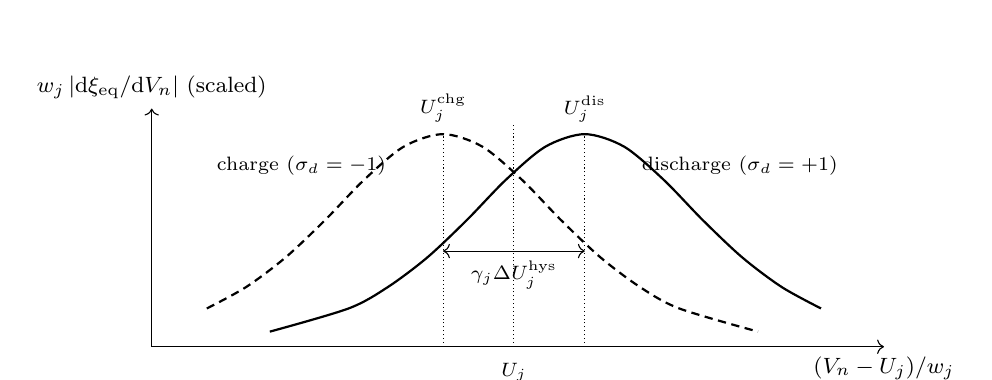
\begin{tikzpicture}[x=1.0cm,y=2.7cm]
\draw[->] (-4.6,0) -- (4.7,0) node[below] {\footnotesize $(V_n-U_j)/w_j$};
\draw[->] (-4.6,0) -- (-4.6,1.12) node[above] {\footnotesize $w_j\,|\dd\xi_\eq/\dd V_n|$ (scaled)};
% discharge bell, center shifted to +g (g = +0.9 here as illustration)
\draw[thick] plot[smooth] coordinates {(-3.1,0.071) (-2.1,0.180) (-1.6,0.281) (-1.1,0.420) (-0.6,0.595) (-0.1,0.786) (0.4,0.941) (0.9,1.0) (1.4,0.941) (1.9,0.786) (2.4,0.595) (2.9,0.420) (3.4,0.281) (3.9,0.180)};
% charge bell, center shifted to -g
\draw[thick,densely dashed] plot[smooth] coordinates {(-3.9,0.180) (-3.4,0.281) (-2.9,0.420) (-2.4,0.595) (-1.9,0.786) (-1.4,0.941) (-0.9,1.0) (-0.4,0.941) (0.1,0.786) (0.6,0.595) (1.1,0.420) (1.6,0.281) (2.1,0.180) (3.1,0.071)};
\draw[densely dotted] (0,0) -- (0,1.05); \node[below] at (0,-0.03) {\scriptsize $U_j$};
\draw[densely dotted] (0.9,0) -- (0.9,1.0); \node[above] at (0.9,1.01) {\scriptsize $U_j^\dis$};
\draw[densely dotted] (-0.9,0) -- (-0.9,1.0); \node[above] at (-0.9,1.01) {\scriptsize $U_j^\chg$};
\draw[<->] (-0.9,0.45) -- (0.9,0.45) node[pos=0.5,below] {\scriptsize $\gamma_j\Delta U_j^\hys$};
\node[right] at (1.5,0.85) {\scriptsize discharge ($\sigma_d=+1$)};
\node[left] at (-1.5,0.85) {\scriptsize charge ($\sigma_d=-1$)};
\end{tikzpicture}
\caption{히스테리시스 분기~\eqref{eq:hyscenter}. 평형 종(N6)의 중심이 방전은 $U_j^\dis=U_j+\tfrac12\gamma_j\Delta U_j^\hys$ 로 위로, 충전은 $U_j^\chg$ 로 아래로 갈린다(여기 $\gamma_j\Delta U_j^\hys=1.8\,w_j$ 예시). 두 중심차가 $\gamma_j\Delta U_j^\hys$. 종의 모양$\cdot$면적은 방향 공통이고 중심만 $\sigma_d$ 로 옮겨진다. $\gamma_j\to0$ 또는 $\Omega_j\le2RT$ 면 두 종이 $U_j$ 에서 겹쳐 본론으로 환원.}
\label{fig:branch}
\end{figure}

\medskip
\emph{넘김.} N3 은 평형 종의 중심을 방향별로 갈랐다($U_j\to U_j^d$). 여기까지가 $|I|\to0$ 평형 구조의 전부다. 다음 N7--N8 은 유한 전류가 이 종에 다는 동역학 꼬리를 — 먼저 지연 길이(N7), 그 길이로 인과 합성곱(N8) — 닫는다.

% ====================================================================
\section{N7 — 동역학 지연 길이 $L_V$}\label{sec:tail}
% ====================================================================
유한 전류에서 전이 진행은 평형 목표를 뒤따라가지 못하고 뒤처진다 — 그 지연이 peak 의 꼬리다. 이 절은 꼬리의 특성 길이 $L_V$ 를 닫는다. 코드의 \code{\_resolve\_lag\_length} 가 전이당 \emph{상수} $L_V$ 를 한 번 산출하고(대표 $T_\rep$$\cdot$대표 $n$), 그 안에서 \code{func\_L\_q}$\cdot$\code{func\_chi\_d}$\cdot$\code{func\_dH\_a\_eff} 를 호출한다. 평형 중심$\cdot$폭은 N2--N5 에서 받았다.

\subsection{지연의 보편 방정식과 길이 $L_q$}
정전류 방전에서 $\dd q/\dd t=|I|/Q_\cell$ 이다. 운동방정식은 N5 의 정$\cdot$역 속도 차를 완화 속도 $k_j\equiv r_j^++r_j^-$(다음 소절에서 Eyring 으로 닫는다)로 묶은 $\dd\xi_j/\dd t=k_j(\xi_{\eq,j}-\xi_j)$ 다. 이를 $\dd q/\dd t$ 로 나누면 진행률의 용량 미분이 나오고, 지연 $r_j\equiv\xi_{\eq,j}-\xi_j$ 의 변화율은 영역 제한 없는 보편 방정식이 된다:
\begin{equation}
\frac{\dd r_j}{\dd q}=\frac{\dd\xi_{\eq,j}}{\dd q}-\frac{r_j}{L_{q,j}},\qquad
\boxed{\;L_{q,j}=\frac{|I|}{Q_\cell\,k_j}\;.}
\label{eq:Lq}
\end{equation}
첫 항은 목표 이동의 지연 \emph{공급}, 둘째 항은 완화의 지연 \emph{소거}다. $L_{q,j}$ 는 요구 $|I|/Q_\cell$ 와 공급 $k_j$ 의 비 그 자체로, 근본식 세 인자가 전부 이 한 양을 통해 꼬리로 들어온다.

\subsection{완화 속도 $k_j$ — Eyring 과 유효 장벽}
완화 속도는 전이상태 이론의 속도식을 따른다 \cite{eyring1935} — 시도 빈도 $k_0=k_BT/h$ 에 Boltzmann 인자를 곱한 형:
\begin{equation}
k\simeq k_0\exp\!\Big[-\frac{\Delta G_a}{RT}\Big],\qquad k_0=\frac{k_BT}{h},\qquad \Delta G_a=\Delta H_a-T\Delta S_a.
\label{eq:eyring}
\end{equation}
정$\cdot$역을 다 세우면 완화 속도의 보편형은 정방향에 역방향 몫을 더한 형이다 — detailed balance~\eqref{eq:db} 의 $r_j^-=r_j^+e^{-\mathcal A_j/RT}$ 로
\begin{equation}
k_j=r_j^++r_j^-=k_0\exp\!\Big[-\frac{\Delta G_{a,j}-\chi_d\mathcal A_j}{RT}\Big]\big(1+e^{-\mathcal A_j/RT}\big).
\label{eq:kuniv}
\end{equation}
꼬리는 구동력 $\mathcal A_j>0$ 이라 정방향이 우세하고($\mathcal A_j\gtrsim3RT$ 면 괄호 인자 $\to1$, 역방향 몫 $e^{-\mathcal A_j/RT}\lesssim5\%$), 그 극한이 forward 형이다:
\begin{equation}
k_j\simeq k_0\exp\!\Big[-\frac{\Delta G_{a,j}-\chi_d\,\mathcal A_j}{RT}\Big].
\label{eq:keff}
\end{equation}
$\chi_d$ 는 방향형 전달 계수다(아래). $L_{q,j}\propto1/k_j$ 를 식~\eqref{eq:Lq} 로 쓰고 보편형~\eqref{eq:kuniv} 의 괄호 인자까지 살려 $k_0=k_BT/h$ 를 넣어 로그를 취하면 — 괄호 인자가 $-\ln(1+e^{-\mathcal A/RT})$ 로 내려와 — 코드 \code{func\_L\_q} 의 줄이 닫힌다:
\begin{equation}
\boxed{\;\ln L_{q,j}=\ln\frac{T_*}{T}-\ln\!\big(1+e^{-\mathcal A/RT}\big)+\frac{\Delta G_{a,j}^\eff}{RT}-\frac{\chi_d\,\mathcal A}{RT}\;,\qquad
T_*=\frac{|I|\,h}{Q_\cell\,k_B}\;.}
\label{eq:lnLq}
\end{equation}
여기서 $\Delta G_{a,j}^\eff=\Delta H_{a,j}^\eff-T\Delta S_{a,j}$, $T_*$ 는 로그 무차원화 특성 온도다. 코드 대응 — \code{T\_attempt}$=T_*$, \code{dG\_a}$=\Delta G_a^\eff$, \code{x}$=\chi_d$, \code{A}$=\mathcal A$. 괄호 인자 $-\ln(1+e^{-\mathcal A/RT})$ 가 N5 의 보편형 $(1+e^{-\mathcal A/RT})$ 를 되살린다($\mathcal A$ 가 깊으면 $\to0$).

\subsection{컷 affinity $\mathcal A$ — 꼬리 시작점의 구동력}
꼬리는 평형 종 $\dd\xi_\eq/\dd V_n=\sigma_d\xi_\eq(1-\xi_\eq)/w$(N6 식~\eqref{eq:dxidV})이 정점($\tfrac14$) 아래로 충분히 떨어지는 컷에서 시작한다. 그 컷의 구동력은 진행률 정규화 변수 $z=\mathcal A/(nRT)$ 가 고정값 $z_\mathrm{cut}$ 에 닿는 점이고, 발산 방지를 위해 상한을 둔다:
\begin{equation}
\boxed{\;\mathcal A=\min\!\big(z_\mathrm{cut}\,n\,RT,\ \ A_\mathrm{cap}\,RT\big)\;.}
\label{eq:Acut}
\end{equation}
기본값 $z_\mathrm{cut}=4.357$ 은 종 $\xi_\eq(1-\xi_\eq)$ 가 정점값 $\tfrac14$ 의 $5\%$ 로 떨어지는 컷이다($\xi_\eq(1-\xi_\eq)/\tfrac14\big|_{z=4.357}\approx0.05$; 이때 점유 자체는 $\xi_\eq\approx0.987$). 상한 배수 $A_\mathrm{cap}=4.0$. 부호 주의 — $\mathcal A$ 는 \emph{크기}라 충$\cdot$방전 동일($\sigma_d$ 가 $\min$ 밖에 안 들어감). 방향은 아래 $\chi_d$$\cdot\Delta H_a^\eff$ 가 받는다. 코드 주석이 명시하듯, 원본의 $\min(s\cdot\dots,4RT)$ 처럼 $\sigma_d$ 를 $\min$ 안에 두면 충전에서 음수 상한이 되던 버그를 정정한 형태다.

\subsection{방향형 $\chi_d$ 와 유효 장벽 $\Delta H_a^\eff$}
전달 계수는 detailed balance 의 합-1 강제(N5 식~\eqref{eq:db})에서 방향별로 거울 대칭이다:
\begin{equation}
\boxed{\;\chi_d=\begin{cases}\chi & \sigma_d\ge0\ (\text{방전})\\ 1-\chi & \sigma_d<0\ (\text{충전})\end{cases}}
\label{eq:chid}
\end{equation}
이것이 \code{func\_chi\_d} 다(생성자 \code{chi\_split} 로 교체 가능 — 기본 규칙). 방전 깊은 꼬리는 $\xi\to1$, 충전은 $\xi\to0$ 거울이라 역방향 장벽의 상수 몫이 갈린다. 깊은 꼬리에서 구동력의 상호작용 몫 $-\Omega_j(1-2\xi_j)$ 를 떼면 상수 $+\Omega_j$ 가 활성화 엔탈피에 흡수되어, 유효 장벽이
\begin{equation}
\boxed{\;\Delta H_{a,j}^\eff=\Delta H_{a,j}-\chi_d\,\Omega_j\;}
\label{eq:dHeff}
\end{equation}
다(\code{func\_dH\_a\_eff}). 방향별($\chi_d$)이라 충$\cdot$방전 꼬리 길이가 갈린다. 코드는 \code{use\_dH\_eff} 로 이 보강을 켜고 끈다(기본 켬).

\subsection{$L_q\to L_V$ — 전압축으로}
용량축 길이를 전압축으로 옮기려면 컷점의 OCV 기울기를 곱한다:
\begin{equation}
\boxed{\;L_{V,j}=\Big|\frac{\dd V_n}{\dd q}\Big|_{q_a}\,L_{q,j}\;.}
\label{eq:LV}
\end{equation}
코드의 \code{dVdq\_qa} 가 $|\dd V/\dd q|_{q_a}$ 다(전이 dict 입력 — 저율 OCV 또는 GITT \cite{weppner1977} 로 측정). 지연 길이 산출에는 우회로 둘이 있다 — (i) \code{L\_V} 직접 지정이 있으면 그대로 쓰고(피팅$\cdot$테스트), (ii) $|I|\le0$ 또는 동역학 키(\code{dH\_a}) 부재면 $L_V=0$(평형 종, 꼬리 없음). 그 외에는 식~\eqref{eq:Acut}$\to$\eqref{eq:lnLq}$\to$\eqref{eq:LV} 를 순서대로 평가한다.

\begin{boundbox}
\textbf{전위 의존의 부호.} 식~\eqref{eq:lnLq} 을 $V_n$ 으로 미분하면 affinity~\eqref{eq:affinity} $\mathcal A_j=\sigma_dF(V_n-U_j)$ 를 통해 $\partial\ln L_{q,j}/\partial V_n=-\chi_d\sigma_dF/RT\le0$($\sigma_d=+1$ 방전 기준) — 구동이 깊을수록 꼬리가 짧아진다(``전위$\uparrow\Rightarrow$꼬리$\downarrow$''). 이 부호가 ★부호 체크리스트 6번이다. 선형 근사 작동 창은 $3RT\lesssim\mathcal A_j\ll\lambda$(Marcus 재구성 에너지)이고, 삽입 상전이의 $\lambda$ 는 수십 kJ/mol 이라 넉넉하다 \cite{marcus1956}.
\end{boundbox}

\begin{codebox}
\code{\_resolve\_lag\_length} 호출 순서: \code{A = min(z\_cut*n\_safe*R*T, A\_cap*R*T)} → \code{chi\_d, dH\_a\_use = \_chi\_and\_dH\_eff(...)} → \code{L\_q = func\_L\_q(T, I, Q\_cell, dH\_a\_use, dS\_a, chi\_d, A)} → \code{return abs(dVdq\_qa) * L\_q}. $n_\mathrm{safe}=|n|$ 로 크기만 쓴다. \code{z\_cut}$\cdot$\code{A\_cap\_RT}$\cdot$\code{use\_dH\_eff} 는 전이별 override 가능(전역 기본 덮어쓰기).
\end{codebox}

\medskip
\emph{넘김.} N7 은 전이당 상수 지연 길이 $L_V$ 를 산출했다. 다음 N8 은 이 $L_V$ 로 평형 점유를 인과 저역통과시켜 실제 지연 점유 $\xi_\lag$ 를 만들고, 그 차 $(\xi_\eq-\xi_\lag)/L_V$ 가 꼬리 달린 peak 가 된다 — 충전은 격자 역전으로 처리한다.

% ====================================================================
\section{N8 — 인과 기억 꼬리와 충전 격자 역전}\label{sec:memory}
% ====================================================================
이 절은 지연 길이 $L_V$(N7)를 써서 실제 관측 peak 모양을 만든다. 핵심은 지연이 ``진행 방향의 과거''만 기억하는 인과(causal) 과정이라는 것이고, 충전은 진행 방향이 방전과 반대라 격자를 뒤집어 처리한다 — ★부호 사슬 7번. 코드의 \code{\_causal\_lowpass} 와 전이 루프의 N8 분기가 대응한다.

\subsection{지연의 일반해 — 지수 기억}
보편 방정식~\eqref{eq:Lq} 는 1계 선형 ODE 라 적분인자 $e^{q/L_q}$ 로 닫힌 해를 갖는다. $q_0$ 부터 적분하면 지연은 초기값의 지수 감쇠와 과거 목표 변화율의 지수 가중 합(합성곱)이다:
\begin{equation}
r_j(q)=r_j(q_0)\,e^{-(q-q_0)/L_{q,j}}+\int_{q_0}^{q}e^{-(q-q')/L_{q,j}}\,\frac{\dd\xi_{\eq,j}}{\dd q'}\,\dd q'.
\label{eq:memory}
\end{equation}
계는 용량축에서 길이 $L_{q,j}$ 만큼의 최근 과거만 기억한다. 이산화하면 지연 점유 $\xi_\lag$ 는 평형 점유 $\xi_\eq$ 의 지수 저역통과(1-pole IIR)다 — 격자 한 칸 $g_\mathrm{step}$ 당 감쇠
\begin{equation}
a=\exp\!\Big(-\frac{g_\mathrm{step}}{L_V}\Big),\qquad
\xi_\lag[i]=a\,\xi_\lag[i-1]+(1-a)\,\xi_\eq[i].
\label{eq:lowpass}
\end{equation}
이것이 \code{\_causal\_lowpass} 다(scipy \code{lfilter} 계수 $b=[1-a]$, $a_\mathrm{coef}=[1,-a]$; 초기 상태 $a\,\xi_\eq[0]$). $L_V\to0$ 이면 $a\to0$ 이라 $\xi_\lag\to\xi_\eq$(지연 없음), $L_V\to\infty$ 면 $a\to1$ 이라 강하게 평활(긴 꼬리).

\subsection{peak 모양 — 평형에서 지연을 뺀 것}
관측 ICA 기여는 ``평형 점유에서 지연 점유를 뺀 것''을 길이로 나눈 것이다:
\begin{equation}
\boxed{\;\text{peak\_shape}_j=\frac{\xi_{\eq,j}-\xi_{\lag,j}}{L_{V,j}}\;.}
\label{eq:peakshape}
\end{equation}
이것이 닫힌식~\eqref{eq:closed}(N9)에서 평형 항과 지연 항을 한꺼번에 담는 이산형이다. $L_V$ 가 격자 분해능 이하($L_V<m_\lag\,g_\mathrm{step}$, \code{min\_lag\_grid\_steps}$=2$)면 코드는 합성곱을 건너뛰고 평형 종~\eqref{eq:eqcontrib} 을 직접 쓴다($\xi_\lag\approx\xi_\eq$ 의 미분 극한 — N6 평형 peak 로 환원). 이것이 ``$L_V$ 작으면 평형 peak 환원''(★부호 체크리스트의 환원 검산)이다.

\subsection{충전 격자 역전 — 진행 방향의 과거}
인과 합성곱~\eqref{eq:lowpass} 은 격자 인덱스 증가 방향을 ``과거$\to$현재''로 본다. 방전($\sigma_d=+1$)은 진행이 $V$ \emph{증가} 방향이라 격자 오름차순이 곧 진행 순서다 — 그대로 필터한다. 충전($\sigma_d=-1$)은 진행이 $V$ \emph{감소} 방향이라 진행 순서가 격자와 반대다. 그래서 코드는 격자를 뒤집어 필터한 뒤 되돌린다:
\begin{equation}
\boxed{\;\xi_\lag=\begin{cases}
\mathrm{lowpass}(\xi_\eq,\,g_\mathrm{step},\,L_V) & \sigma_d\ge0\ (\text{방전})\\[2pt]
\mathrm{lowpass}(\xi_\eq[::\!-\!1],\,g_\mathrm{step},\,L_V)[::\!-\!1] & \sigma_d<0\ (\text{충전})
\end{cases}\;}
\label{eq:reversal}
\end{equation}
즉 충전은 \code{occ\_lagged = \_causal\_lowpass(ksi\_arr[::-1], grid\_step, lag\_len\_V)[::-1]}. 이 역전이 꼬리를 진행 방향(충전은 저전위 쪽)으로 향하게 해, 충전 $\dd Q/\dd V$ 가 방전의 거울이면서도 양수를 유지하게 한다(그림~\ref{fig:reversal}). 역전을 빠뜨리면 충전 꼬리가 엉뚱한 쪽으로 뻗어 부호$\cdot$모양이 모두 깨진다.

\begin{figure}[t]
\centering
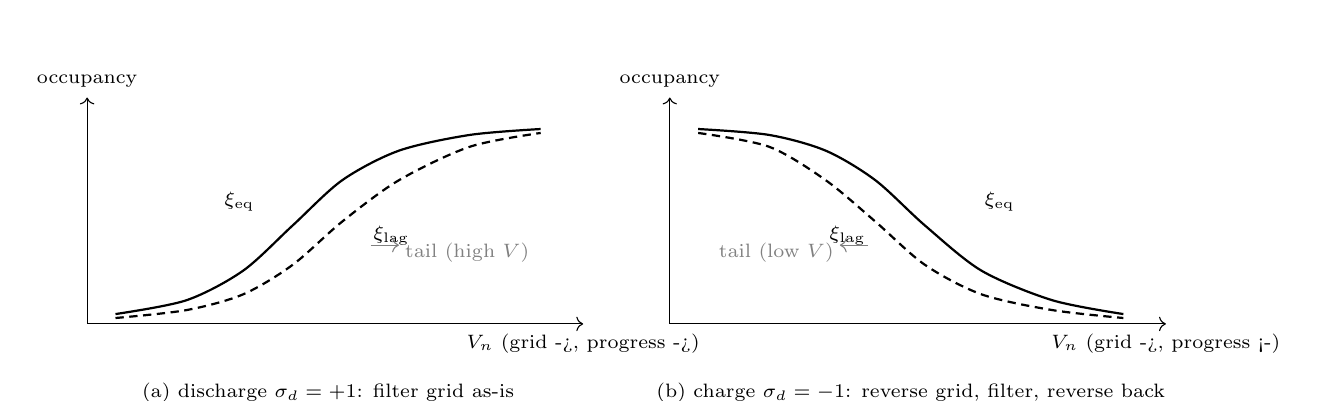
\begin{tikzpicture}[x=0.90cm,y=2.5cm]
% --- discharge panel ---
\begin{scope}
\draw[->] (-3.4,0) -- (3.6,0) node[below] {\scriptsize $V_n$ (grid ->, progress ->)};
\draw[->] (-3.4,0) -- (-3.4,1.15) node[above] {\scriptsize occupancy};
% xi_eq logistic rising
\draw[thick] plot[smooth] coordinates {(-3,0.05) (-2,0.12) (-1.2,0.27) (-0.5,0.5) (0.2,0.73) (1,0.88) (2,0.96) (3,0.99)};
% xi_lag: lagged to the right (delayed in progress = higher V)
\draw[thick,densely dashed] plot[smooth] coordinates {(-3,0.03) (-2,0.07) (-1.2,0.15) (-0.5,0.30) (0.2,0.52) (1,0.73) (2,0.90) (3,0.97)};
\draw[->,gray] (0.6,0.40) -- (1.0,0.40);
\node[gray,right] at (0.95,0.36) {\scriptsize tail (high $V$)};
\node[right] at (-1.6,0.62) {\scriptsize $\xi_\eq$};
\node[right] at (0.5,0.45) {\scriptsize $\xi_\lag$};
\node at (0,-0.35) {\scriptsize (a) discharge $\sigma_d=+1$: filter grid as-is};
\end{scope}
% --- charge panel ---
\begin{scope}[xshift=7.4cm]
\draw[->] (-3.4,0) -- (3.6,0) node[below] {\scriptsize $V_n$ (grid ->, progress <-)};
\draw[->] (-3.4,0) -- (-3.4,1.15) node[above] {\scriptsize occupancy};
% xi_eq logistic: charge sigma_d=-1, rises toward LOW V. Show xi_eq decreasing with V
\draw[thick] plot[smooth] coordinates {(-3,0.99) (-2,0.96) (-1.2,0.88) (-0.5,0.73) (0.2,0.5) (1,0.27) (2,0.12) (3,0.05)};
% xi_lag: lagged in progress direction (progress is toward low V) -> lag is toward HIGH V side, i.e. tail on low V
\draw[thick,densely dashed] plot[smooth] coordinates {(-3,0.97) (-2,0.90) (-1.2,0.73) (-0.5,0.52) (0.2,0.30) (1,0.15) (2,0.07) (3,0.03)};
\draw[->,gray] (-0.6,0.40) -- (-1.0,0.40);
\node[gray,left] at (-0.95,0.36) {\scriptsize tail (low $V$)};
\node[left] at (1.6,0.62) {\scriptsize $\xi_\eq$};
\node[left] at (-0.5,0.45) {\scriptsize $\xi_\lag$};
\node at (0,-0.35) {\scriptsize (b) charge $\sigma_d=-1$: reverse grid, filter, reverse back};
\end{scope}
\end{tikzpicture}
\caption{인과 지연과 충전 격자 역전~\eqref{eq:reversal}. (a) 방전은 진행이 $V$ 증가 방향이라 격자 그대로 저역통과 — 지연 $\xi_\lag$(파선)가 진행의 뒤(높은 $V$)에 처지고 꼬리가 그쪽으로 뻗는다. (b) 충전은 진행이 $V$ 감소 방향이라 격자를 뒤집어 필터 후 되돌린다 — 꼬리가 거울처럼 낮은 $V$ 쪽으로 뻗는다. 두 경우 모두 $\text{peak\_shape}=(\xi_\eq-\xi_\lag)/L_V$ 가 양수다(방전의 거울 $=$ 충전, 부호 유지).}
\label{fig:reversal}
\end{figure}

\medskip
\emph{넘김.} N8 은 전이별 peak 모양(평형 종 또는 꼬리 달린 종)을 완성했다. 마지막 N9 이 전이별 기여 $Q_j\cdot\text{peak\_shape}_j$ 를 배경 위에 합산하고 측정축으로 되돌린다.

% ====================================================================
\section{N9 — 합산$\cdot$역보간과 닫힌식}\label{sec:summation}
% ====================================================================
전이 루프가 끝나면 각 전이의 기여를 합산해 한 곡선으로 닫는다. 합산이 \emph{선형}인 것은 가정이 아니라 전하 보존의 직접 결과다 — 빠진 리튬이 전이별 몫의 합이라($Q_\cell\,q=Q_\bg+\sum_j Q_j\xi_j$), 양변을 $V_n$ 으로 미분하면 ICA 가 전이별 기여의 합이 된다. 앞 절들의 peak\_shape 를 받아 이 절이 곡선을 완성한다.

\subsection{닫힌식 — 평형에서 지연을 뺀 것의 미분}
작업 격자 위 합산과 역보간(측정축 복귀)이 N9 다:
\begin{equation}
\boxed{\;\frac{\dd Q}{\dd V_n}\;=\;C_\bg\;+\;\sum_{j=1}^{N_p}Q_j\,\frac{\xi_{\eq,j}-\xi_{\lag,j}}{L_{V,j}}
\;=\;C_\bg+\sum_{j=1}^{N_p}Q_j\big[\text{평형 peak}-\text{지연 꼬리}\big]\;.}
\label{eq:closed}
\end{equation}
``임의 접합''이 아니라 평형 점유에서 지연을 뺀 것의 미분이라는 정의 형태다. 코드의 마지막 두 줄이 이것이다 — 루프 안에서 \code{dqdv\_work += Q\_j * peak\_shape}, 루프 뒤 \code{dqdv\_out = np.interp(V\_n, V\_work, dqdv\_work)}. 역보간이 작업 격자(꼬리 여유 포함)의 곡선을 측정 전위 $V_n$ 격자로 되돌린다. 스칼라 입력이면 첫 원소를 반환한다.

\subsection{두 극한 — 환원 검산}
닫힌식~\eqref{eq:closed} 은 두 극한에서 정확히 환원된다(★부호 체크리스트 정합):
\begin{equation}
\frac{\dd Q}{\dd V_n}\;\xrightarrow{\ L_V\to0\ }\;
C_\bg+\sum_j Q_j\,\frac{\xi_{\eq,j}(1-\xi_{\eq,j})}{w_j}
\;=\;\code{equilibrium()},
\label{eq:reduce}
\end{equation}
곧 $|I|\to0$ 또는 빠른 동역학에서 N6 평형 peak 기준선(식~\eqref{eq:equilcode})으로 복귀한다. 그리고 $\gamma_j=0$ 또는 $\Omega_j\le2RT$ 면 분기 중심이 단일 $U_j$ 로 합쳐져, $|I|\to0$ 에서 충$\cdot$방전 두 곡선이 완전히 겹친다(히스는 상분리의 산물). 충전 곡선은 N1$\cdot$N3$\cdot$N8 의 세 $\sigma_d$ 작용을 거쳐 방전의 거울이면서 양수를 유지한다.

\subsection{staging 전이 초기값 — 재현 가능성 표}\label{sec:stagingtable}
곡선을 실제로 그리려면 전이 목록과 인자 초기값이 필요하다. 코드의 \code{GRAPHITE\_STAGING\_LIT} 가 흑연 네 전이의 시작값이다 — \emph{신뢰값이 아니라 피팅 override 전제의 초기값}이다(열역학은 $U(298)$ 정합, $\Delta H_a$ 는 DFT 경향, $\Omega$ 는 추정).

\begin{table}[t]
\centering
\renewcommand{\arraystretch}{1.25}
\begin{tabular}{l c c c c c c c}
\toprule
전이(stage) & $U$\,[V] & $\Delta H_\rxn$ & $\Delta S_\rxn$ & $Q$ & $\Omega$ & $\Delta H_a$ & $\dd V/\dd q|_{q_a}$ \\
 & ($w$\,[V]) & [kJ/mol] & [J/mol/K] & [$Q_\cell$] & [kJ/mol] & [kJ/mol] & [V] \\
\midrule
$4\!\to\!3$    & 0.210 (0.020) & $-11.7$ & $+29.0$ & 0.10 & 6.0  & 48.0 & 0.30 \\
$3\!\to\!2\mathrm L$ & 0.140 (0.016) & $-13.5$ & $0.0$   & 0.12 & 8.0  & 46.0 & 0.30 \\
$2\mathrm L\!\to\!2$ & 0.120 (0.014) & $-13.1$ & $-5.0$  & 0.25 & 10.0 & 44.0 & 0.30 \\
$2\!\to\!1$    & 0.085 (0.012) & $-13.0$ & $-16.0$ & 0.50 & 13.0 & 40.0 & 0.30 \\
\bottomrule
\end{tabular}
\caption{\code{GRAPHITE\_STAGING\_LIT} 전이 초기값(코드와 1:1; $\dd S_a=0$, $n=1$). $U$ 는 폴백(하위호환) 직접 중심이고 $\Delta H_\rxn/\Delta S_\rxn$ 가 $U(298)$ 을 재현한다(N2 검산). $Q$ 는 $Q_\cell$ 정규화 — 만충 stage $2\!\to\!1$ 이 최대용량 $0.50$. $\Omega$ 는 정규용액 상호작용(stage 깊을수록 증가), $\Delta H_a$ 는 DFT 활성화(만충쪽 감소 경향), $\dd V/\dd q|_{q_a}$ 는 컷 OCV 기울기($L_q\!\to\!L_V$ 환산). 전부 초기값이며 실제 값은 데이터가 정한다.}
\label{tab:staging}
\end{table}

\begin{verifybox}
\textbf{재현 가능성(G-usable) — 이 문건만으로 곡선 짜기.} (1) 표~\ref{tab:staging} 로 모델 생성, 전역 인자 $\chi=x$(기본 $0.5$), $R_n$, $C_\bg$, \code{use\_dH\_eff}(기본 True), \code{use\_w\_eff}(기본 False), $z_\mathrm{cut}=4.357$, $A_\mathrm{cap}=4.0$. (2) 조건 $(V_\app,\sigma_d,|I|,Q_\cell,T)$. (3) N1: $V_n=V_\app-\sigma_d|I|R_n$, 작업 격자~\eqref{eq:vwork}. (4) 전이마다 N2 $U_j(T)$~\eqref{eq:Uj} → N3 $U_j^d$~\eqref{eq:hyscenter}($\gamma\ne0$ 일 때) → N4 $w$~\eqref{eq:weff} → N5 $\xi_\eq$~\eqref{eq:logistic} → N7 $L_V$(식~\eqref{eq:Acut}$\to$\eqref{eq:lnLq}$\to$\eqref{eq:LV}) → N8 $\xi_\lag$~\eqref{eq:reversal} 및 $\text{peak\_shape}$~\eqref{eq:peakshape}($L_V<2g_\mathrm{step}$ 면 평형 종~\eqref{eq:eqcontrib}). (5) N9 합산~\eqref{eq:closed} 후 역보간. \textbf{검산값} — stage $2\!\to\!1$ 중심 $U(298)\approx0.085$ V; $\Omega_j=2RT$ 에서 $\Delta U^\hys=0$; $|I|\to0$ 에서 방$\cdot$충 곡선 일치($\gamma=0$). 코드의 \code{\_\_main\_\_} self-test 가 이 값들을 검증한다.
\end{verifybox}

\subsection{전체 진행 한눈에 — N0 에서 N9 까지}
그림~\ref{fig:flow} 가 한 곡선을 그리는 전 과정이다. 절 순서가 곧 이 흐름이다.

\begin{figure}[t]
\centering
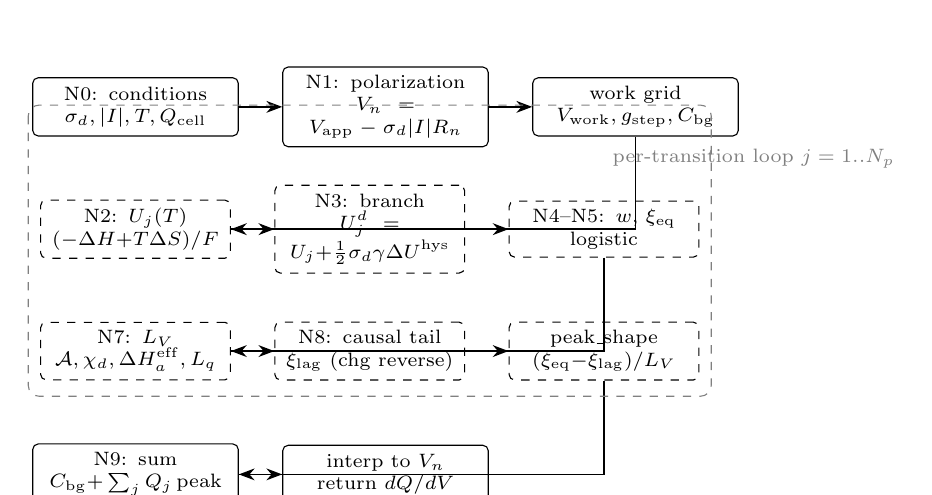
\begin{tikzpicture}[
  node distance=3.3mm and 5.5mm,
  box/.style={draw,rounded corners=2pt,minimum height=7.4mm,inner sep=3pt,font=\scriptsize,align=center,text width=24mm},
  loopbox/.style={draw,dashed,rounded corners=2pt,minimum height=7.0mm,inner sep=3pt,font=\scriptsize,align=center,text width=22mm},
  ar/.style={-{Stealth[length=2mm]},semithick}]
\node[box] (n0) {N0: conditions\\$\sigma_d,|I|,T,Q_\cell$};
\node[box,right=of n0] (n1) {N1: polarization\\$V_n=V_\app-\sigma_d|I|R_n$};
\node[box,right=of n1] (grid) {work grid\\$V_\work,g_\mathrm{step},C_\bg$};
\draw[ar] (n0)--(n1); \draw[ar] (n1)--(grid);
% transition loop boxes
\node[loopbox,below=8mm of n0] (n2) {N2: $U_j(T)$\\$(-\Delta H{+}T\Delta S)/F$};
\node[loopbox,right=of n2] (n3) {N3: branch\\$U_j^d=U_j{+}\tfrac12\sigma_d\gamma\Delta U^\hys$};
\node[loopbox,right=of n3] (n45) {N4--N5: $w$, $\xi_\eq$\\logistic};
\draw[ar] (n2)--(n3); \draw[ar] (n3)--(n45);
\node[loopbox,below=8mm of n2] (n7) {N7: $L_V$\\$\mathcal A,\chi_d,\Delta H_a^\eff,L_q$};
\node[loopbox,right=of n7] (n8) {N8: causal tail\\$\xi_\lag$ (chg reverse)};
\node[loopbox,right=of n8] (ps) {peak\_shape\\$(\xi_\eq{-}\xi_\lag)/L_V$};
\draw[ar] (n45) |- (n7); \draw[ar] (n7)--(n8); \draw[ar] (n8)--(ps);
\node[box,below=8mm of n7] (n9) {N9: sum\\$C_\bg{+}\sum_j Q_j\,$peak};
\node[box,right=of n9] (out) {interp to $V_n$\\return $dQ/dV$};
\draw[ar] (ps) |- (n9); \draw[ar] (n9)--(out);
\draw[ar] (grid) |- (n2);
% loop label
\node[font=\scriptsize,gray] at ($(n45)+(1.9,0.9)$) {per-transition loop $j=1..N_p$};
\draw[gray,dashed,rounded corners] ($(n2.north west)+(-0.15,1.2)$) rectangle ($(ps.south east)+(0.15,-0.2)$);
\end{tikzpicture}
\caption{한 곡선을 그리는 계산 진행 $N0\!\to\!N9$(코드 \code{curve}$\to$\code{dqdv}). 위 줄 = 조건 환산$\cdot$분극$\cdot$작업 격자(N0--N1). 점선 상자 = 전이별 루프(N2--N8): 평형 중심$\to$분기$\to$폭$\cdot$점유$\to$지연 길이$\to$인과 꼬리$\to$peak 모양. 아래 줄 = 합산과 측정축 역보간(N9). 본 장의 절 순서가 이 흐름과 1:1.}
\label{fig:flow}
\end{figure}

\medskip
\emph{도착.} 한 줄 합산식~\eqref{eq:closed} 과 그 모든 기호의 코드 식별자$\cdot$초기값(표~\ref{tab:staging})$\cdot$산출 순서(그림~\ref{fig:flow})가 닫혔다. 곡선을 데이터에 맞추는 비순환 피팅 사슬 — 저율 OCV 로 $\{U_j,w_j,Q_j,C_\bg\}$, 전류 차단으로 $R_n$, 다전위 꼬리로 $\chi$, 다온도로 $\Delta H_a^\eff$, 다율 gap 으로 $\{\gamma_j,\Omega_j\}$ 를 단계마다 한 겹씩 동결 — 은 같은 닫힌식의 기호를 측정 파일에서 정하는 절차이며, 본 장의 식들이 그 각 단계의 모델 함수를 그대로 제공한다.

% ====================================================================
\begin{thebibliography}{99}
\bibitem{dahn1991} J. R. Dahn, ``Phase diagram of Li$_x$C$_6$,'' \emph{Phys. Rev. B} \textbf{44}, 9170 (1991). DOI: 10.1103/PhysRevB.44.9170.
\bibitem{ohzuku1993} T. Ohzuku, Y. Iwakoshi, K. Sawai, ``Formation of Lithium-Graphite Intercalation Compounds in Nonaqueous Electrolytes,'' \emph{J. Electrochem. Soc.} \textbf{140}, 2490 (1993). DOI: 10.1149/1.2220849.
\bibitem{funabiki1999} A. Funabiki, M. Inaba, Z. Ogumi et al., ``Stage Transformation of Lithium-Graphite Intercalation Compounds Caused by Electrochemical Lithium Intercalation,'' \emph{J. Electrochem. Soc.} \textbf{146}, 2443 (1999). DOI: 10.1149/1.1391953.
\bibitem{bazant2013} M. Z. Bazant, ``Theory of Chemical Kinetics and Charge Transfer based on Nonequilibrium Thermodynamics,'' \emph{Acc. Chem. Res.} \textbf{46}, 1144 (2013). DOI: 10.1021/ar300145c.
\bibitem{eyring1935} H. Eyring, ``The Activated Complex in Chemical Reactions,'' \emph{J. Chem. Phys.} \textbf{3}, 107 (1935). DOI: 10.1063/1.1749604.
\bibitem{marcus1956} R. A. Marcus, ``On the Theory of Oxidation-Reduction Reactions Involving Electron Transfer. I,'' \emph{J. Chem. Phys.} \textbf{24}, 966 (1956). DOI: 10.1063/1.1742723.
\bibitem{evanspolanyi1938} M. G. Evans, M. Polanyi, ``Inertia and driving force of chemical reactions,'' \emph{Trans. Faraday Soc.} \textbf{34}, 11 (1938). DOI: 10.1039/TF9383400011.
\bibitem{bardfaulkner} A. J. Bard, L. R. Faulkner, \emph{Electrochemical Methods: Fundamentals and Applications}, 2nd ed., Wiley (2001). ISBN 978-0-471-04372-0.
\bibitem{dreyer2010} W. Dreyer \emph{et al.}, ``The thermodynamic origin of hysteresis in insertion batteries,'' \emph{Nature Materials} \textbf{9}, 448 (2010). DOI: 10.1038/nmat2730.
\bibitem{reynier2004} Y. Reynier, R. Yazami, B. Fultz, ``Thermodynamics of Lithium Intercalation into Graphites and Disordered Carbons,'' \emph{J. Electrochem. Soc.} \textbf{151}, A422 (2004). DOI: 10.1149/1.1646152.
\bibitem{weppner1977} W. Weppner, R. A. Huggins, ``Determination of the Kinetic Parameters of Mixed-Conducting Electrodes (GITT),'' \emph{J. Electrochem. Soc.} \textbf{124}, 1569 (1977). DOI: 10.1149/1.2133112.
\bibitem{dubarry2012} M. Dubarry, C. Truchot, B. Y. Liaw, ``Synthesize battery degradation modes via a diagnostic and prognostic model,'' \emph{J. Power Sources} \textbf{219}, 204 (2012). DOI: 10.1016/j.jpowsour.2012.07.016.
\bibitem{bloom2005} I. Bloom, A. N. Jansen, D. P. Abraham et al., ``Differential voltage analyses of high-power, lithium-ion cells. 1. Technique and application,'' \emph{J. Power Sources} \textbf{139}, 295 (2005). DOI: 10.1016/j.jpowsour.2004.07.021.
\end{thebibliography}

\end{document}
